\chapter{Introdução}
\label{cap:introducao}
 
 
Em 1958 surgia o primeiro jogo eletrônico com o nome de "Tênis para dois", criado pelo físico William Higinbotham.O jogo era processado por um computador analógico e exibido em um osciloscópio.
\cite{mass}


Em 1961 um grupo de estudantes do MIT desenvolveram o jogo Spacewar! No jogo o objetivo era que os jogadores controlassem suas naves num ambiente escuro tentando abater o adversário. O jogo era desenvolvido num grande computador, que ocupava o espaço de uma sala inteira, o DEC PDP-1, este computador tinha como objetivo executar cálculos em geral porém apos o jogo Spacewar! o computador ficou famoso pela possibilidade de entreter outros. \cite{ram}


Foi então em 1972 que o primeiro jogo comercial foi lançado pela Atari, o Pong, ilustrado na figura 1. Era um jogo simples e intuitivo, características que o fez ser tao popular para a época. \cite{tracc} 

\begin{figure}[h!]
		\centering
		\Caption{\label{fig:exemplo-1}Jogo Pong criado pela Atari em 1972}	
		\UECEfig{}{
			\fbox{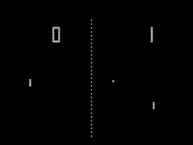
\includegraphics[width=7cm]{figuras/193px-Pong}}
		}{
			\Fonte{Wikipedia, 2015}			
		}	
	\end{figure}


Estes citados foram os responsáveis pela grande diversidade e popularidade que os jogos alcançam ultimamente.

Atualmente devido a popularização da internet e dos dispositivos móveis, em destaque o uso de \textit{smartphones} no qual evidenciado na pesquisa realizada pela consultoria Nielsen, 68 milhões de brasileiros utilizam \textit{smartphones} \cite{nie} 

Tendo em base a estatística da Nielsen, as palavras do diretor geral da Pontomobi, Renato Virgilli, tornam-se ainda mais expressivas diz ele: "Com o número cada vez maior de celulares, de \textit{smartphones} e de \textit{tablets} nas mãos dos usuários, cresce o interesse por aplicativos, seja para diversão ou entretenimento". \cite{vir}

Ainda de acordo com a empresa Flurry do grupo Yahoo, o uso de aplicativos cresceu em média 76\% em 2014. \cite{prox}
	
	
Os aplicativos da categoria jogos tornaram-se um passatempo global, dados comprovados na pequisa  realizada pela empresa Flurry, informando que os jogadores globais (plataforma Android) gastam em media 37 minutos por dia jogando. Desses 37 minutos, a categoria que prevalece é a de jogos casuais. \cite{flur}

Uma das vias para qual o mercado de aplicativos de jogos tem mostrado desenvolvimento eficiente é como ferramenta pedagógica.
"O aluno é totalmente ativo ao usar um aplicativo, diferente de uma TV, que ele tem uma postura mais passiva. Os envolvidos no processo passam de consumidores a produtores de conteúdo, e a ter mais autonomia e criatividade, habilidades que serão demandadas no seu futuro profissional".

Considerações essa de Tori, coordenador do Laboratório de Tecnologias Interativas da USP (Universidade de São Paulo) de que o aplicativo tem a capacidade de auxiliar o desenvolvimento de uma tarefa, e que a escola não pode viver numa realidade desconectada da do aluno.

A professora e diretora-executiva do Instituto Educadigital, Priscila Gonsales vem com o conceito de que recurso digitais e audiovisuais auxiliam a interação e visualização, aponta também que o aplicativo não substitui a metodologia tradicional e a utilização da ferramenta deva ser contextual ao conteúdo abordado. \cite{tori}

Baseando-se nos itens descritos acima: popularidade no uso de aplicativos e que este tem eficiência no uso didático, foi desenvolvido e sera apresentado neste documento o jogo digital Caapora, que tem como objetivo ensinar crianças sobre a importância da preservação da mata e ressaltar a cultura folclórica brasileira.
Aplicativo este desenvolvido para uso em  dispositivos móveis com sistema operacional Android.

\section{Motivação}
\label{cap:motivacao}

A floresta amazônica faz parte do ecossistema do mundo, é fundamental para o equilíbrio climático e é conhecida por ser o pulmão do mundo. Faz parte de 9 países dentre eles Brasil, Bolívia, Peru, Colômbia, Equador e Venezuela. E contém metade dos animais terrestres do planeta.

Apesar da extensão e de sua importância, a floresta Amazônica sofre uma grande degradação causada pelo desmatamento predatório e ilegal, poluição de rios, desequilíbrio em sua fauna e flora e em vezes ocorrendo a expulsão a força de populações nativas de seus territórios.

Em uma recente pesquisa da ONG Instituto do Homem e do Meio Ambiente da Amazônia (Imazon) do Pará, o aumento do desmatamento cresceu mais de 400\% em comparação a novembro de 2013. \cite{des}

Outra grande riqueza que a Amazônia brasileira possui, é a sua grande diversidade de cultura, na parte que engloba a Amazônia brasileira (Acre, Amapá, Amazonas, Pará, Rondônia, Roraima e parte dos estados do Mato Grosso, Tocantins e Maranhão) tem-se os contos folclóricos, que segundo a carta do Folclore Brasileiro \cite{fc}, folclore é o conjunto das criações culturais de uma comunidade, baseado nas suas tradições expressas individual ou coletivamente, representativo de sua identidade social.

Em grande parte dos contos folclóricos os personagens são criaturas místicas tendo alguns deles o objetivo de proteger a floresta e as criaturas nela habitadas.


Um exemplo deste personagem é o Caipora (Caapora, em tupi, significa habitante do mato \cite{sig}), vive montado em um porco do mato e é conhecido por espantar os madeireiros com seu assobio, ajudar animais presos em armadilhas e aprontar travessuras, com o objetivo de espantar os que estão fazendo mal a mãe natureza. 

Segundo Franchini, o caipora é conhecido por várias regiões do brasil, mas a sua forma física e seu método de ação varia de acordo com a região.
Na figura 2 é possível ver dois tipos diferentes em que se acreditam que o Caipora possa existir, em um ele é uma figura feminina e em outro é um menino-índio montado em um porco do mato. \cite{100}

\begin{figure}[h!]
		\centering
		\Caption{\label{fig:exemplo-4}Diversidade de formas da Caipora}	
		\UECEfig{}{
			\fbox{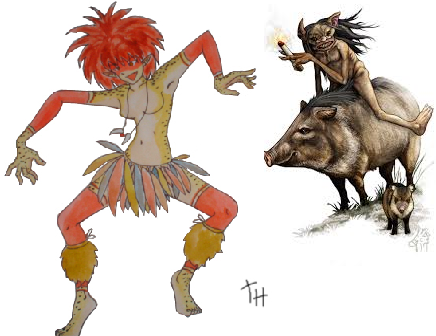
\includegraphics[width=7cm]{figuras/caipora5}}
		}{
			\Fonte{\cite{cp1}}			
		}	
	\end{figure}